%=============================================================
%  PLANTILLA – Manual de Prácticas
%  Universidad de Cuenca · Facultad de Ingeniería
%  Diseño basado en el Libro de Marca UCUENCA
%
%  USO: copiar esta carpeta completa, renombrarla, y editar
%       (1) los datos del documento (bloque DATOS DEL DOCUMENTO),
%       (2) los capítulos .tex, y (3) references.bib.
%  Compilar con:  latexmk -pdf -outdir=build main.tex
%=============================================================
\documentclass[12pt,a4paper,oneside,openany]{book}
% Evitar páginas en blanco que book inserta entre partes
\let\cleardoublepage=\clearpage

%=============================================================
%  DATOS DEL DOCUMENTO  (se usan en portada, encabezado y PDF)
%=============================================================
% Título de la portada (usar \\ para partir líneas)
\newcommand{\DocTitulo}{Manual de\\[4pt]Prácticas}
% Línea destacada bajo el título (equipo / tema / asignatura)
\newcommand{\DocTema}{Impresora 3D Robo R2}
% Línea pequeña bajo el tema (opcional; dejar vacío si no se usa)
\newcommand{\DocSubtitulo}{Guía práctica de uso para estudiantes}
% Autor y afiliación
\newcommand{\DocAutor}{Ing.\ Nombre Apellido}
\newcommand{\DocDepartamento}{Departamento de Ingeniería Eléctrica, Electrónica y Telecomunicaciones}
\newcommand{\DocLugarAnio}{Cuenca\,--\,Ecuador \quad 2026}
% Texto del encabezado de cada página (se pasa a mayúsculas)
\newcommand{\DocEncabezado}{Manual de Prácticas -- Impresora 3D Robo R2}
% Metadatos del PDF (sin comandos LaTeX)
\newcommand{\DocTituloPDF}{Manual de Prácticas -- Impresora 3D Robo R2}
\newcommand{\DocAutorPDF}{Nombre Apellido}

%=============================================================
%  Plantilla UCUENCA – Configuración de formato
%  Manual de Prácticas · Universidad de Cuenca
%  Diseño basado en el Libro de Marca UCUENCA
%
%  Este archivo NO debería editarse por documento: los datos
%  propios (título, autor, encabezado) se definen en main.tex.
%=============================================================

%-------------------------------------------------------------
% ENCODING & LANGUAGE
%-------------------------------------------------------------
\usepackage[utf8]{inputenc}
\usepackage[T1]{fontenc}
\usepackage{csquotes}
\usepackage{babel}
\babelprovide[import,main]{spanish}

%-------------------------------------------------------------
% FONTS
% FiraSans (humanista sans, acorde al Libro de Marca UCUENCA)
%-------------------------------------------------------------
\usepackage[sfdefault,light]{FiraSans}
\usepackage{FiraMono}
\usepackage{microtype}

%-------------------------------------------------------------
% PAGE LAYOUT
%-------------------------------------------------------------
\usepackage[top=2.8cm, bottom=2.8cm, left=3cm, right=2.5cm,
            headheight=16pt]{geometry}

%-------------------------------------------------------------
% GRAPHICS & COLOR
%-------------------------------------------------------------
\usepackage{graphicx}
\graphicspath{{images/}}
\usepackage[dvipsnames,table]{xcolor}

%-------------------------------------------------------------
% BRAND COLORS  (Libro de Marca UCUENCA, pp. 26-27)
%-------------------------------------------------------------
\definecolor{UCblue}{RGB}{0,40,86}
\definecolor{UCred}{RGB}{165,16,8}
\definecolor{UCgris}{RGB}{111,111,111}
\definecolor{UCbluelight}{RGB}{230,236,244}
\definecolor{UCbluemid}{RGB}{0,62,126}
\definecolor{codebg}{RGB}{248,248,248}
\definecolor{infoboxbg}{RGB}{232,240,252}
\definecolor{successgreen}{RGB}{39,174,96}
\definecolor{warnyellow}{RGB}{241,196,15}

%-------------------------------------------------------------
% COLORES DE CÓDIGO ARDUINO
%-------------------------------------------------------------
\definecolor{arduino}{HTML}{00A3A9}
\definecolor{astructure}{HTML}{818A42}
\definecolor{avariables}{HTML}{128F8F}
\definecolor{afunctions}{HTML}{DB6B21}
\definecolor{aback}{HTML}{E0E0E2}
\definecolor{amyblue}{rgb}{0.01,0.61,0.98}
\definecolor{amygray}{rgb}{0.47,0.47,0.33}

%-------------------------------------------------------------
% TABLES
%-------------------------------------------------------------
\usepackage{booktabs}
\usepackage{tabularx}
\usepackage{multirow}
\usepackage{array}
\usepackage{longtable}
\usepackage{xltabular}

%-------------------------------------------------------------
% HEADERS & FOOTERS
%-------------------------------------------------------------
\usepackage{fancyhdr}
\usepackage{lastpage}

%-------------------------------------------------------------
% LISTS
%-------------------------------------------------------------
\usepackage{enumitem}
\newcommand{\keys}[1]{%
  {\small\normalfont\sffamily\fboxsep=2pt\fbox{\vphantom{Xy}#1}}}
\newcommand{\ctrl}{Ctrl}
\newcommand{\alt}{Alt}
\newcommand{\shift}{Shift}

%-------------------------------------------------------------
% CODE LISTINGS
%-------------------------------------------------------------
\usepackage{listings}
\usepackage{tcolorbox}
\tcbuselibrary{listings, skins, breakable}

%-------------------------------------------------------------
% MATH
%-------------------------------------------------------------
\usepackage{amsmath,amssymb}

%-------------------------------------------------------------
% HYPERLINKS
%-------------------------------------------------------------
\usepackage[colorlinks=true,
            linkcolor=UCblue,
            urlcolor=UCblue,
            citecolor=UCblue,
            bookmarks=true,
            unicode=true,
            pdftitle={\DocTituloPDF},
            pdfauthor={\DocAutorPDF}]{hyperref}

%-------------------------------------------------------------
% BIBLIOGRAPHY
%-------------------------------------------------------------
\usepackage[backend=biber,style=ieee]{biblatex}
\addbibresource{references.bib}

%-------------------------------------------------------------
% MISC
%-------------------------------------------------------------
\usepackage{caption}
\usepackage{subcaption}
\usepackage{float}
\usepackage{mdframed}
\usepackage{titlesec}
\usepackage{titletoc}
\usepackage{pifont}
\usepackage{fontawesome5}
\usepackage{tikz}
\usetikzlibrary{shapes.geometric,arrows.meta,positioning,shadows,
                fit,backgrounds,calc,shapes,arrows}
\usepackage{comment}

%=============================================================
%  ESTILO DE LISTADOS (Arduino / C++)
%=============================================================
\newcommand*{\FormatDigit}[1]{\ttfamily\textcolor{black}{#1}}
\lstdefinestyle{FormattedNumber}{%
    literate=*{0}{{\FormatDigit{0}}}{1}%
             {1}{{\FormatDigit{1}}}{1}%
             {2}{{\FormatDigit{2}}}{1}%
             {3}{{\FormatDigit{3}}}{1}%
             {4}{{\FormatDigit{4}}}{1}%
             {5}{{\FormatDigit{5}}}{1}%
             {6}{{\FormatDigit{6}}}{1}%
             {7}{{\FormatDigit{7}}}{1}%
             {8}{{\FormatDigit{8}}}{1}%
             {9}{{\FormatDigit{9}}}{1}%
             {.0}{{\FormatDigit{.0}}}{2}%
             {.1}{{\FormatDigit{.1}}}{2}%
             {.2}{{\FormatDigit{.2}}}{2}%
             {.3}{{\FormatDigit{.3}}}{2}%
             {.4}{{\FormatDigit{.4}}}{2}%
             {.5}{{\FormatDigit{.5}}}{2}%
             {.6}{{\FormatDigit{.6}}}{2}%
             {.7}{{\FormatDigit{.7}}}{2}%
             {.8}{{\FormatDigit{.8}}}{2}%
             {.9}{{\FormatDigit{.9}}}{2}%
             {\ }{{ }}{1},%
}

\lstset{%
  basicstyle=\footnotesize\ttfamily,
  breakatwhitespace=false,
  breaklines=true,
  captionpos=b,
  commentstyle=\color{UCgris},
  deletekeywords={...},
  escapeinside={\%*}{*)},
  extendedchars=true,
  keepspaces=true,
  keywordstyle=[1]\color{astructure},
  keywordstyle=[2]\color{avariables},
  keywordstyle=[3]\color{afunctions},
  keywordstyle=[4]\bfseries\color{afunctions},
  language=c++,
  morekeywords={*,...},
  numbers=left,
  numbersep=5pt,
  numberstyle=\tiny\color{amygray},
  rulecolor=\color{black},
  rulesepcolor=\color{amyblue},
  showspaces=false,
  showstringspaces=false,
  showtabs=false,
  tabsize=2,
  title=\lstname,
  emphstyle=\color{avariables},
  frame=single,
  framexleftmargin=15pt,
  rulecolor=\color{arduino},
  literate=%
    {á}{{\'{a}}}1 {é}{{\'{e}}}1 {í}{{\'{i}}}1 {ó}{{\'{o}}}1 {ú}{{\'{u}}}1
    {Á}{{\'{A}}}1 {É}{{\'{E}}}1 {Í}{{\'{I}}}1 {Ó}{{\'{O}}}1 {Ú}{{\'{U}}}1
    {ñ}{{\~{n}}}1 {Ñ}{{\~{N}}}1
}

\lstdefinestyle{Arduino}{%
    style=FormattedNumber,
    keywords={setup, loop, if, else, for, switch, while, do, break, continue, return, goto},
    morekeywords=[2]{HIGH, LOW, INPUT, OUTPUT, INPUT_PULLUP, LED_BUILTIN, true, false,
                     int, float, void, boolean, char, word, long, short, double, string, array},
    morekeywords=[3]{const, pinMode, digitalWrite, digitalRead, analogReference, analogRead,
                     analogWrite, analogReadResolution, analogWriteResolution, tone, noTone,
                     shiftOut, shiftIn, pulseIn, millis, micros, delay, delayMicroseconds,
                     min, max, abs, constrain, map, pow, sqrt, sin, cos, tan, randomSeed,
                     random, lowByte, highByte, bitRead, bitWrite, bitSet, bitClear, bit,
                     attachInterrupt, detachInterrupt, interrupts, noInterrupts,
                     Stream, Keyboard, Mouse, begin, println, print},
    morekeywords=[4]{Serial},
    morecomment=[l]{//},
    morecomment=[s]{/*}{*/},
    emph={const},
}

% Entorno para bloques de código Arduino:
%   \begin{ArduinoSketchBox}{Título del sketch} ... \end{ArduinoSketchBox}
\newtcblisting{ArduinoSketchBox}[2][]{
  colframe=arduino,
  enhanced, drop shadow, sharp corners, boxrule=1pt,
  width=\dimexpr\linewidth+\parindent\relax,
  left skip=-\parindent,
  arc=3pt, outer arc=3pt,
  listing only,
  listing options={
    frame=,
    style=Arduino,
  },
  title=#2,
  #1
}

% Enlace externo (ícono)
\newcommand{\ExternalLink}{%
    \tikz[x=1.2ex, y=1.2ex, baseline=-0.05ex]{%
        \begin{scope}[x=1ex, y=1ex]
            \clip (-0.1,-0.1)
                --++ (-0, 1.2)
                --++ (0.6, 0)
                --++ (0, -0.6)
                --++ (0.6, 0)
                --++ (0, -1);
            \path[draw,
                line width = 0.5,
                rounded corners=0.5]
                (0,0) rectangle (1,1);
        \end{scope}
        \path[draw, line width = 0.5] (0.5, 0.5) -- (1, 1);
        \path[draw, line width = 0.5] (0.6, 1) -- (1, 1) -- (1, 0.6);
        }
    }

% Enlace con nota al pie:  \doclink{URL}{texto visible}
\newcommand{\doclink}[2]{\href{#1}{#2}\footnote{\url{#1}}}

%=============================================================
%  TCOLORBOX STYLES (plantilla UCUENCA)
%  objetivebox · materialbox · infobox · warningbox · entregabox
%=============================================================
\newtcolorbox{objetivebox}{
  enhanced, breakable,
  colback=UCbluelight,
  colframe=UCblue,
  fonttitle=\bfseries\small\color{white},
  title={\faBookOpen\hspace{5pt}Objetivos de Aprendizaje},
  arc=2pt,
  left=8pt, right=8pt, top=6pt, bottom=6pt,
  boxrule=0pt, titlerule=0pt,
  attach boxed title to top left={yshift=-2pt,xshift=0pt},
  boxed title style={colback=UCblue, arc=2pt, boxrule=0pt},
}

\newtcolorbox{materialbox}{
  enhanced, breakable,
  colback=white,
  colframe=UCred,
  fonttitle=\bfseries\small\color{white},
  title={\faTools\hspace{5pt}Materiales y Equipos},
  arc=2pt,
  left=8pt, right=8pt, top=6pt, bottom=6pt,
  boxrule=0pt,
  attach boxed title to top left={yshift=-2pt},
  boxed title style={colback=UCred, arc=2pt, boxrule=0pt},
}

\newtcolorbox{infobox}[1][Nota]{
  enhanced, breakable,
  colback=infoboxbg,
  colframe=UCblue,
  fonttitle=\bfseries\small,
  title={\faInfoCircle\hspace{5pt}#1},
  arc=2pt, boxrule=0.6pt,
  left=8pt, right=8pt, top=4pt, bottom=4pt,
}

\newtcolorbox{warningbox}[1][Advertencia]{
  enhanced, breakable,
  colback=warnyellow!15,
  colframe=warnyellow!70!black,
  fonttitle=\bfseries\small,
  title={\faExclamationTriangle\hspace{5pt}#1},
  arc=2pt, boxrule=0.6pt,
  left=8pt, right=8pt, top=4pt, bottom=4pt,
}

\newtcolorbox{entregabox}{
  enhanced, breakable,
  colback=successgreen!8,
  colframe=successgreen!70!black,
  fonttitle=\bfseries\small\color{white},
  title={\faClipboardCheck\hspace{5pt}Entregables},
  arc=2pt, boxrule=0pt,
  attach boxed title to top left={yshift=-2pt},
  boxed title style={colback=successgreen!70!black, arc=2pt, boxrule=0pt},
  left=8pt, right=8pt, top=6pt, bottom=6pt,
}

%=============================================================
%  CHAPTER & SECTION FORMATTING  (estilo Libro de Marca)
%=============================================================
\titleformat{\chapter}[display]
  {\normalfont\LARGE\bfseries\color{UCblue}}
  {\color{UCred}\large\bfseries\chaptername\ \thechapter}
  {4pt}
  {}
  [{\color{UCblue}\vspace{-4pt}\rule{\linewidth}{2pt}}]
\titlespacing*{\chapter}{0pt}{-20pt}{28pt}

\titleformat{\section}
  {\normalfont\large\bfseries\color{UCblue}}
  {\thesection}{1em}{}
  [{\color{UCred}\vspace{1pt}\rule{\linewidth}{1.5pt}}]

\titleformat{\subsection}
  {\normalfont\normalsize\bfseries\color{UCred}}
  {\thesubsection}{1em}{}

\titleformat{\subsubsection}
  {\normalfont\normalsize\bfseries\color{UCblue}}
  {\thesubsubsection}{1em}{}

%=============================================================
%  HEADER / FOOTER  (estilo Libro de Marca UCUENCA)
%=============================================================
\pagestyle{fancy}
\fancyhf{}
\fancyhead[L]{%
  \footnotesize\bfseries\color{UCred}\MakeUppercase{\DocEncabezado}}
\fancyhead[R]{%
  \footnotesize\bfseries\color{UCblue}\MakeUppercase{Universidad de Cuenca}}
\fancyfoot[R]{\small\color{UCgris}\thepage}
\renewcommand{\headrulewidth}{0.4pt}
\renewcommand{\footrulewidth}{0pt}

\fancypagestyle{plain}{
  \fancyhf{}
  \fancyfoot[R]{\small\color{UCgris}\thepage}
  \renewcommand{\headrulewidth}{0pt}
}

%=============================================================
%  MACROS DE UTILIDAD
%=============================================================
\newcommand{\pinref}[1]{\texttt{#1}}
\newcommand{\comp}[1]{\textbf{#1}}

% Tikz settings para diagramas de control
\tikzset{
  block/.style = {draw, fill=white, rectangle, minimum height=3em, minimum width=3em},
  tmp/.style  = {coordinate},
  sum/.style  = {draw, fill=white, circle, node distance=1cm},
  input/.style = {coordinate},
  output/.style= {coordinate},
  pinstyle/.style = {pin edge={to-,thin,black}}
}


% Macros propias de este manual (rutas de menú de la pantalla táctil)
\newcommand{\flecha}{\,$\rightarrow$\,}
\newcommand{\ruta}[1]{\textbf{#1}}
\newcommand{\grados}[1]{#1\,\textdegree C}

%=============================================================
%  DOCUMENT
%=============================================================
\begin{document}

%=============================================================
%  Portada  (estilo Libro de Marca UCUENCA)
%  Los textos se definen en main.tex (\DocTitulo, \DocTema, ...)
%=============================================================
\pagestyle{empty}

\begin{titlepage}
  \thispagestyle{empty}
  \pagecolor{UCblue}
  \color{white}

  \begin{tikzpicture}[remember picture, overlay]
    % Franja roja superior
    \fill[UCred] ([yshift=-3.8cm]current page.north west)
      rectangle ([yshift=-4.2cm]current page.north east);
    % Franja roja inferior
    \fill[UCred] ([yshift=3.6cm]current page.south west)
      rectangle ([yshift=3.2cm]current page.south east);
  \end{tikzpicture}

  % Cabecera UCUENCA
  \vspace*{0.9cm}
  \begin{flushleft}
    {\fontsize{42}{46}\selectfont\bfseries
      \textcolor{white}{U}\textcolor{white}{CUENCA}}\\[-6pt]
    {\color{UCred}\rule{0.52\linewidth}{3pt}}\\[4pt]
    {\small\bfseries\color{white!80!UCblue}\MakeUppercase{Ingeniería}}
  \end{flushleft}

  \vspace{3.8cm}

  % Título principal
  \begin{flushleft}
    {\fontsize{38}{44}\selectfont\bfseries\color{white}%
      \DocTitulo}\\[10pt]
    {\fontsize{22}{26}\selectfont\bfseries\color{white!85!UCblue}%
      \DocTema}\\[6pt]
    {\small\color{white!60!UCblue}\DocSubtitulo}
  \end{flushleft}

  \vfill

  % Autor
  \begin{flushleft}
    {\color{UCred}\rule{0.4\linewidth}{1pt}}\\[8pt]
    {\normalsize\bfseries\color{white}%
      \DocAutor}\\[4pt]
    {\small\color{white!70!UCblue}%
      \DocDepartamento}\\[16pt]
    {\footnotesize\color{white!50!UCblue}%
      \DocLugarAnio}
  \end{flushleft}

  \vspace{0.6cm}
\end{titlepage}

% Restaurar color de página
\pagecolor{white}\color{black}
\pagestyle{fancy}


%-------------------------------------------------------------
%  TABLA DE CONTENIDOS
%-------------------------------------------------------------
\tableofcontents
\clearpage

%=============================================================
%  CONTENIDO
%=============================================================
\chapter{Introducción}

La \textbf{Robo R2} es una impresora 3D de tipo FDM (modelado por deposición fundida): funde filamento plástico y construye la pieza capa por capa. Este manual resume, para uso en el laboratorio, lo esencial del manual del fabricante~\cite{robomanual}: cómo ponerla en marcha, calibrarla, imprimir una pieza, controlarla a distancia y mantenerla en buen estado.

El flujo de trabajo es siempre el mismo: se diseña o descarga un modelo (\texttt{.stl}), un programa \textbf{laminador} (Cura for Robo) lo convierte en instrucciones (\texttt{.gcode}) y la impresora las ejecuta desde su pantalla táctil, una memoria USB o el panel web.

\begin{figure}[H]
    \centering
    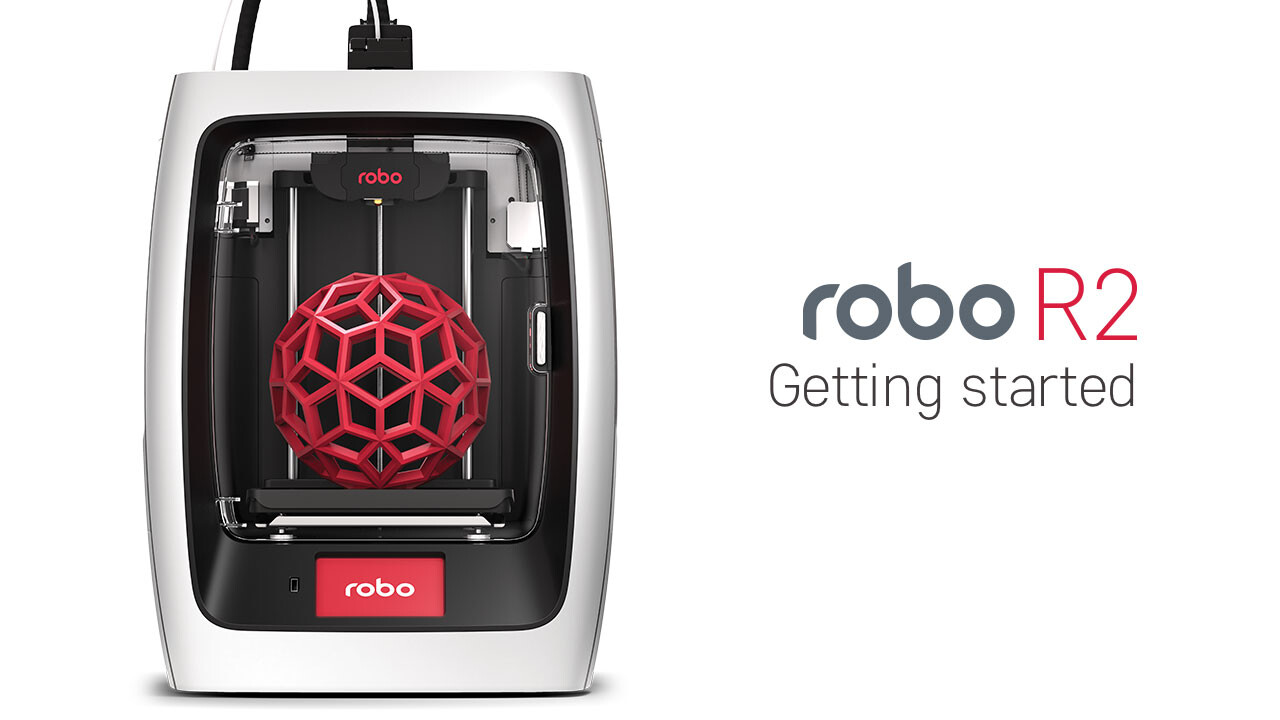
\includegraphics[width=0.55\linewidth]{r2_inicio.jpg}
    \caption{Impresora Robo R2 (imagen del manual del fabricante~\cite{robomanual}).}
    \label{fig:r2}
\end{figure}

\section{Contenido de la caja}

Además de la impresora, la caja incluye:

\begin{itemize}
    \item Guía de inicio rápido y voucher de un año del software Autodesk Fusion~360.
    \item Fuente de alimentación de 24~V y tubo guía del filamento.
    \item Caja de herramientas: tapa del hotend, 2 llaves allen, lubricante, pinzas y tarjeta de calibración del Z-Offset.
    \item Memoria USB de Robo, 300~g de filamento (celeste) y espátula.
\end{itemize}

\begin{figure}[H]
    \centering
    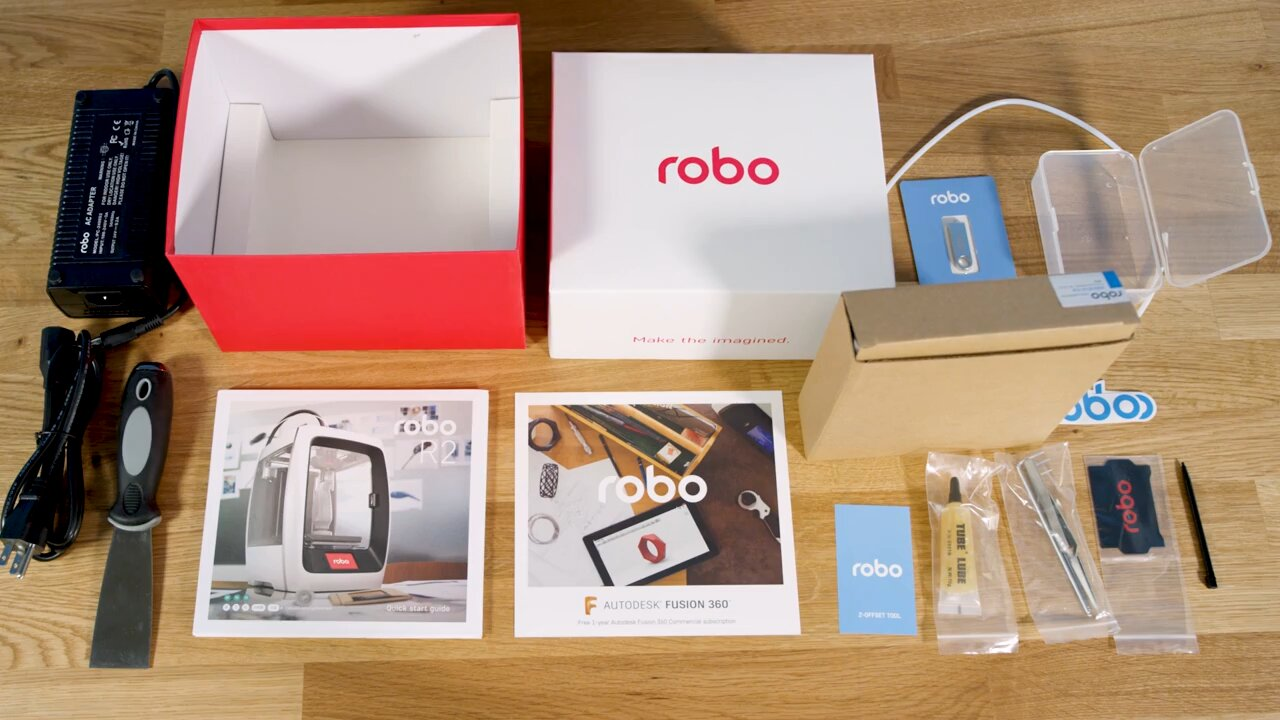
\includegraphics[width=0.7\linewidth]{r2_caja.jpg}
    \caption{Accesorios que vienen con la impresora.}
    \label{fig:caja}
\end{figure}

\section{La pantalla táctil}

La pantalla táctil a color es el punto de acceso principal: se maneja con el dedo o con un lápiz táctil. Tiene tres pestañas:

\begin{description}[leftmargin=2.2cm,style=nextline]
    \item[Files] Archivos de la memoria interna o de una USB.
    \item[Printer] Pantalla de impresión: archivo en curso, temperaturas, progreso, mensajes de error y botones Pause y Cancel.
    \item[Utilities] Ventiladores, asistentes (Wizards), red, actualización y opciones.
\end{description}

\begin{figure}[H]
    \centering
    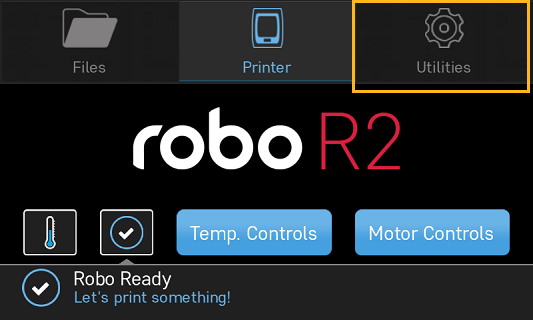
\includegraphics[width=0.48\linewidth]{r2_pantalla_inicio.png}\hfill
    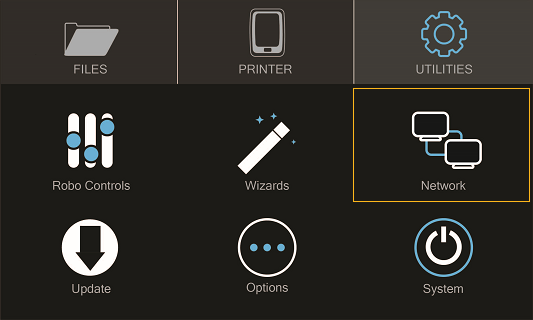
\includegraphics[width=0.48\linewidth]{r2_utilities.png}
    \caption{Pantalla de inicio (izquierda) y menú \emph{Utilities} (derecha).}
    \label{fig:pantallas}
\end{figure}

\section{Seguridad}

\begin{warningbox}[Lea esto antes de usar la impresora]
\begin{itemize}
    \item \textbf{Quemaduras:} el hotend puede llegar a unos \grados{300} y la cama a unos \grados{110}. No toque el hotend con las manos; si es necesario, use las pinzas y espere al menos 30 minutos a que se enfríe.
    \item \textbf{Partes móviles:} no meta la mano ni objetos dentro de la impresora cuando esté en marcha, a punto de arrancar o en reposo.
    \item \textbf{No la deje sola} durante una impresión y apáguela al terminar.
    \item \textbf{Electricidad:} use solo el cable original, con buena conexión a tierra. Todo mantenimiento se hace con la impresora apagada y desenchufada. No modifique la electrónica.
    \item \textbf{Ventilación:} el plástico fundido emite olor; trabaje en un lugar ventilado. No ponga comida ni bebida cerca.
    \item Use guantes al retirar las piezas y las herramientas solo para su fin. Mantenga el equipo lejos de líquidos, fuentes de calor y de niños.
\end{itemize}
\end{warningbox}

\section{Estructura del manual}

\begin{itemize}
    \item \textbf{Práctica 1:} puesta en marcha y calibración.
    \item \textbf{Práctica 2:} preparación e impresión de una pieza.
    \item \textbf{Práctica 3:} control remoto con panel web, app y cámara.
    \item \textbf{Capítulo 5:} mantenimiento y solución de problemas.
\end{itemize}


%-------------------------------------------------------------
%  PRÁCTICAS  (una por archivo)
%-------------------------------------------------------------
\chapter{Práctica 1: Puesta en Marcha y Calibración}

\begin{center}
  \small\renewcommand{\arraystretch}{1.3}
  \begin{tabular}{l l l l}
    \textbf{Equipo:}      & Robo R2   &
    \textbf{Actividades:} & 3 \\
    \textbf{Software:}    & Pantalla táctil RoboOS &
    \textbf{Duración:}    & 1,5 horas \\
  \end{tabular}
\end{center}

\section{Introducción}

Antes de la primera impresión hay que dejar la R2 lista: retirar el embalaje, conectarla a la red, actualizarla, calibrar la altura del hotend sobre la cama (\emph{Z-Offset}) y cargar filamento. Una calibración correcta es la causa principal de una buena primera capa; casi todos los problemas de adhesión nacen de un Z-Offset mal ajustado.

\begin{objetivebox}
\begin{itemize}
    \item Desembalar y preparar la impresora para su uso.
    \item Conectar y actualizar la impresora desde la pantalla táctil.
    \item Calibrar el Z-Offset con el asistente de la pantalla.
    \item Cargar filamento con el asistente de carga.
\end{itemize}
\end{objetivebox}

\vspace{6pt}

\begin{materialbox}
\begin{itemize}
    \item Impresora Robo R2 con su fuente, cable y tubo guía del filamento.
    \item Caja de herramientas (tapa del hotend, llaves allen, pinzas, tarjeta de calibración).
    \item Carrete de filamento PLA y tijeras.
    \item Red Wi-Fi o cable Ethernet.
\end{itemize}
\end{materialbox}

\vspace{6pt}

\begin{warningbox}
Con el hotend caliente no toque la boquilla ni el bloque calefactor. Durante la calibración mantenga las manos fuera de la zona de movimiento de la cama.
\end{warningbox}

\newpage
\section{Actividad 1: Desembalaje y configuración inicial}

\begin{enumerate}
    \item Abra las 3 pinzas inferiores de la caja y retire la cubierta superior. Corte la brida que sujeta la puerta y saque la caja de accesorios, retirando antes la cinta azul.
    \item Retire los \textbf{4 sujetadores naranjas} de las varillas (uno por esquina del carro superior) presionando el clip, y corte las bridas que sujetan las varillas a sus soportes.
    \item Quite la cinta azul que sujeta las partes móviles y levante la impresora por las asas inferiores.
    \item Coloque la \textbf{tapa del hotend} (se sujeta con imanes) y conecte el cable de alimentación a la parte trasera y a la red eléctrica.
    \item Encienda la impresora.
    \item Conecte a Wi-Fi: \ruta{Utilities}\flecha\ruta{Network}\flecha\ruta{Configure Wifi}, elija su red, escriba la clave con el teclado en pantalla y pulse \ruta{Connect}. También puede usar un cable Ethernet.
    \item Actualice: \ruta{Utilities}\flecha\ruta{Update}. Si ya está al día, el botón aparece en gris con la leyenda \emph{up to date}. La actualización tarda cerca de un minuto.
\end{enumerate}

\begin{infobox}[Guarde el embalaje]
Conserve la caja y las espumas: pueden hacer falta para el transporte o para hacer válida la garantía. El fabricante recomienda también registrar el equipo para servicio y garantía.
\end{infobox}

\begin{figure}[H]
    \centering
    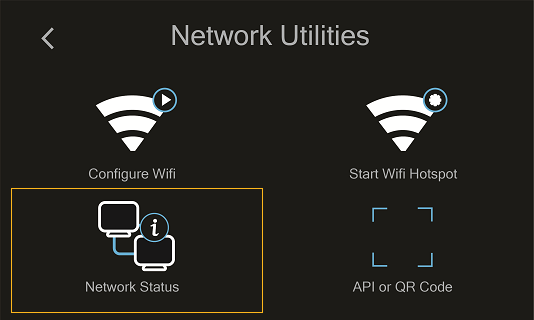
\includegraphics[width=0.5\linewidth]{r2_network.png}
    \caption{Menú \emph{Network Utilities}: configurar Wi-Fi, modo hotspot, estado de red y código QR.}
    \label{fig:network}
\end{figure}

\newpage
\section{Actividad 2: Calibración del Z-Offset}

El \textbf{Z-Offset} es la distancia entre la boquilla y la cama cuando la cama está en su posición de origen (abajo). Puede cambiar si la cama no queda bien asentada o si el hotend se desplaza.

\subsection*{Asistente Z-Offset}

\begin{enumerate}
    \item \ruta{Utilities}\flecha\ruta{Wizards}\flecha\ruta{Z-Offset Wizard}. La impresora se lleva a su posición de origen.
    \item Con las flechas \textbf{arriba/abajo} mueva la cama mientras desliza la \textbf{tarjeta de calibración} (o una hoja de papel) entre la boquilla y la cama.
    \item Deténgase cuando sienta una \textbf{ligera resistencia}: la tarjeta debe poder moverse, pero tocando a la vez la boquilla y la cama. Si la cama está tan alta que la tarjeta no pasa, baje con la flecha hasta que pase con un leve roce.
    \item Pulse \ruta{Finished}; la impresora calcula y guarda el valor. Pulse \ruta{Finished} otra vez para cerrar.
\end{enumerate}

\subsection*{Ajuste fino (Fine Tune Offset)}

Si la boquilla arrastra sobre la cama (Z muy bajo) o la pieza no se pega (Z muy alto), use \ruta{Utilities}\flecha\ruta{Wizards}\flecha\ruta{Fine Tune Offset}. La impresora imprime líneas de prueba y usted sube o baja el valor entre pasadas.

\begin{warningbox}[Antes del ajuste fino]
Nivele la cama con los tornillos de mariposa inferiores antes de iniciar este asistente; de lo contrario, el resultado no es confiable.
\end{warningbox}

\begin{enumerate}
    \item Elija el material cargado y la esquina desde la que empezará a imprimir las líneas.
    \item En la pantalla \emph{Adjust Offset} elija el incremento, use \ruta{Test Offset} y compare con la imagen de referencia.
    \item Cuando el resultado sea satisfactorio, pulse la flecha de avance (arriba a la derecha) y \ruta{Save}.
\end{enumerate}

\begin{infobox}[Ajuste manual (avanzado)]
Se puede editar el valor en \ruta{Utilities}\flecha\ruta{Options}\flecha\ruta{EEPROM}\flecha\ruta{Home Offset}. Un valor \textbf{menor} acerca la cama a la boquilla; uno \textbf{mayor} la aleja. Si el valor es cercano pero la pieza no se pega, pruebe cambios de 0,1 a 0,2~mm.
\end{infobox}

\newpage
\section{Actividad 3: Carga de filamento}

\begin{enumerate}
    \item Desenganche el soporte del carrete empujando la palanca superior desde la parte trasera, e inserte el tubo guía en el bloque del sensor de filamento.
    \item Cuelgue el carrete en el soporte superior, desenrolle al menos \textbf{30~cm} de filamento y \textbf{corte la punta} con tijeras.
    \item Pase el filamento por la base del bloque del sensor y por el tubo guía hasta el extrusor. El filamento \textbf{debe pasar por el bloque del sensor} (si no, el sensor marcará error de falta de filamento).
    \item Presione la palanca del extrusor y guíe el filamento hasta los engranajes.
    \item \ruta{Utilities}\flecha\ruta{Wizards}\flecha\ruta{Filament Loading Wizard}. La impresora calienta; cuando termine, el engranaje empuja el filamento hasta la boquilla.
    \item Cuando vea salir plástico por la boquilla pulse \ruta{Next} y luego \ruta{Done}.
\end{enumerate}

Para \textbf{descargar} el filamento use \ruta{Utilities}\flecha\ruta{Wizards}\flecha\ruta{Filament Change Wizard}: tras calentar, el engranaje retrae el filamento hasta que sale por la parte superior del extrusor.

\begin{infobox}[Cambio de material]
Si cambia de ABS a PLA, caliente el hotend a temperatura de ABS y empuje un poco de PLA para sacar todo el ABS. Después baje a la temperatura del PLA; de lo contrario, la boquilla puede taparse.
\end{infobox}

\section{Entregables}

\begin{entregabox}
\begin{itemize}
    \item Fotografía de la impresora lista (sin sujetadores de embalaje, con tapa del hotend) y captura de la pantalla \emph{up to date}.
    \item Valor de Z-Offset obtenido y breve descripción de cómo se comprobó (tarjeta o papel).
    \item Fotografía del filamento saliendo por la boquilla.
\end{itemize}
\end{entregabox}

\chapter{Práctica 2: Preparación e Impresión de una Pieza}

\begin{center}
  \small\renewcommand{\arraystretch}{1.3}
  \begin{tabular}{l l l l}
    \textbf{Equipo:}      & Robo R2   &
    \textbf{Actividades:} & 3 \\
    \textbf{Software:}    & Cura for Robo &
    \textbf{Duración:}    & 2 horas \\
  \end{tabular}
\end{center}

\section{Introducción}

Para imprimir, el modelo 3D (\texttt{.stl}) debe convertirse en \texttt{.gcode} con un \textbf{laminador}. Cura for Robo es el software recomendado por el fabricante; ya trae perfiles preparados para la R2, de modo que el estudiante solo elige material y calidad. Después el archivo se envía a la impresora por USB o por el panel web.

\begin{objetivebox}
\begin{itemize}
    \item Preparar un modelo en Cura for Robo (material, calidad, orientación y soportes).
    \item Revisar el resultado en la vista de capas antes de imprimir.
    \item Imprimir desde la pantalla táctil y vigilar el progreso.
    \item Retirar la pieza sin dañarla ni dañar la lámina PEI.
\end{itemize}
\end{objetivebox}

\vspace{6pt}

\begin{materialbox}
\begin{itemize}
    \item Robo R2 calibrada y con filamento cargado (Práctica 1).
    \item Computador con Windows de 64 bits y Cura for Robo instalado.
    \item Archivo \texttt{.stl} de la pieza y memoria USB.
    \item Espátula, guantes y paño húmedo.
\end{itemize}
\end{materialbox}

\vspace{6pt}

\begin{infobox}[Temperaturas de referencia]
\begin{center}
\small
\begin{tabular}{l c c}
  \toprule
  \textbf{Material} & \textbf{Hotend} & \textbf{Cama (R2)} \\
  \midrule
  PLA & \grados{190}--\grados{210} & \grados{50} (hasta \grados{70}) \\
  ABS & \grados{230}--\grados{250} & \grados{80} (hasta \grados{100}) \\
  \bottomrule
\end{tabular}
\end{center}
Para el filamento Robo, \grados{190} es el valor óptimo de PLA y \grados{230} el de ABS.
\end{infobox}

\newpage
\section{Actividad 1: Laminar el modelo en Cura for Robo}

Cura for Robo requiere Windows de 64 bits y una tarjeta gráfica compatible con OpenGL~2. La primera vez que lo abra, el asistente pide elegir la impresora: seleccione \textbf{Robo R2} y pulse \ruta{Add Printer}.

\begin{enumerate}
    \item \textbf{Cargar el modelo:} icono \ruta{Open File} (arriba a la izquierda) y elija el \texttt{.stl}.
    \item \textbf{Elegir el material:} debe ser el mismo que está cargado en la impresora.
    \item \textbf{Elegir el perfil:} \emph{Low}, \emph{Medium}, \emph{High} o \emph{Ultra High Quality}. Mayor calidad significa capas más finas y más tiempo de impresión.
    \item \textbf{Ajustes rápidos:} densidad de relleno, adhesión a la cama (\emph{raft}) y estructuras de soporte para voladizos y puentes.
    \item \textbf{Orientar la pieza:} seleccione el modelo y use las herramientas \ruta{Move}, \ruta{Scale} (marque \emph{Uniform Scaling} para conservar proporciones), \ruta{Rotate} (\emph{Lay Flat} la apoya sobre una cara plana) y \ruta{Mirror}.
    \item \textbf{Revisar:} en la vista \emph{Layers} recorra las capas con el deslizador y confirme que la pieza se construye como espera. La vista \emph{X-Ray} marca en rojo huecos e intersecciones del modelo; si aparecen, corríjalos en el programa de diseño.
    \item \textbf{Exportar} el \texttt{.gcode} a la memoria USB.
\end{enumerate}

\begin{table}[H]
    \centering
    \caption{Ajustes de Cura que más influyen en el resultado.}
    \label{tab:cura}
    \small
    \begin{tabularx}{\linewidth}{l X}
        \toprule
        \textbf{Ajuste} & \textbf{Efecto} \\
        \midrule
        Altura de capa & Menor altura: más detalle y más tiempo. Mayor altura: menos detalle y más rápido. \\
        Grosor de paredes & Unas 3 veces el ancho de línea es un valor típico; más paredes dan una pieza más resistente. \\
        Relleno (infill) & Cerca de 20\,\% para piezas visuales; mayor para piezas mecánicas. \\
        Retracción & Reduce los hilos de plástico (stringing). Demasiada retracción puede dañar el filamento o tapar la boquilla. \\
        Velocidad & Los perfiles por defecto equilibran rapidez y vida útil; la primera capa se imprime más lenta para adherir mejor. \\
        \bottomrule
    \end{tabularx}
\end{table}

\newpage
\section{Actividad 2: Imprimir y vigilar}

\subsection*{Iniciar desde la memoria interna}

\begin{enumerate}
    \item En la pantalla de inicio seleccione \ruta{Files} y elija el archivo.
    \item Pulse \ruta{Start} y espere unos segundos mientras la impresora se prepara.
\end{enumerate}

\subsection*{Iniciar desde una memoria USB}

\begin{enumerate}
    \item Inserte la USB en la ranura frontal.
    \item \ruta{Files}\flecha elija el archivo.
    \item Decida si lo copia a la impresora o lo imprime directamente desde la USB.
    \item Pulse \ruta{Start}.
\end{enumerate}

\subsection*{Vigilar la impresión}

La pestaña \ruta{Printer} muestra el nombre del archivo, el porcentaje de avance, el tiempo y las temperaturas. Desde ahí puede pulsar \ruta{Pause} o \ruta{Cancel}, o tocar la temperatura del extrusor para modificarla. También puede seguir el estado desde la app o el panel web (Práctica 3).

\begin{figure}[H]
    \centering
    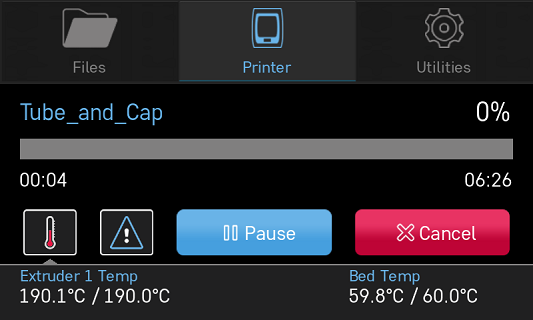
\includegraphics[width=0.55\linewidth]{r2_impresion.png}
    \caption{Pestaña \emph{Printer} durante una impresión: progreso, temperaturas y botones Pause/Cancel.}
    \label{fig:impresion}
\end{figure}

\begin{warningbox}
No deje la impresora sin supervisión y vigile la \textbf{primera capa}: es donde se detectan los problemas de adhesión. Si la boquilla arrastra o el plástico no se pega, cancele y repita la calibración del Z-Offset.
\end{warningbox}

\section{Actividad 3: Retirar la pieza y evaluar}

\begin{enumerate}
    \item Espere a que la pieza y la cama se enfríen.
    \item Retire la cama con las dos manos y colóquela sobre una superficie plana.
    \item Con la espátula, levante la pieza por los bordes y avance poco a poco por debajo. \textbf{No tire de la pieza hacia arriba} desde el centro: puede romperse.
    \item Limpie la lámina PEI con un paño húmedo antes de la siguiente impresión.
    \item Al volver a colocar la cama, verifique que los imanes calcen y que el cable de alimentación de la cama esté conectado: si no está bien asentada, la impresión falla.
\end{enumerate}

\begin{infobox}[Si la pieza ya no se pega]
La lámina PEI dura aproximadamente de 4 a 6 meses. Si las piezas dejan de adherirse, líjela suavemente con lija de grano 2000 y límpiela con un paño húmedo. Luego repita la calibración del Z-Offset.
\end{infobox}

\section{Entregables}

\begin{entregabox}
\begin{itemize}
    \item Captura de Cura for Robo con el modelo, material y perfil elegidos, y de la vista de capas.
    \item Fotografía de la pieza impresa y tiempo total de impresión.
    \item Breve análisis: ¿cómo salió la primera capa? ¿Qué ajuste cambiaría y por qué?
\end{itemize}
\end{entregabox}

\chapter{Práctica 3: Control Remoto (Panel Web, App y Cámara)}

\begin{center}
  \small\renewcommand{\arraystretch}{1.3}
  \begin{tabular}{l l l l}
    \textbf{Equipo:}      & Robo R2   &
    \textbf{Actividades:} & 3 \\
    \textbf{Software:}    & Panel web y app Robo (iOS) &
    \textbf{Duración:}    & 1 hora \\
  \end{tabular}
\end{center}

\section{Introducción}

La R2 puede controlarse sin tocar su pantalla: desde un navegador (panel web) o desde la app Robo para iOS. Esto permite subir archivos, laminar, fijar temperaturas, mover los ejes y ver el interior de la impresora con su cámara integrada. Para todo ello la impresora debe estar conectada a la misma red o en modo hotspot.

\begin{objetivebox}
\begin{itemize}
    \item Conectarse al panel web de la impresora.
    \item Subir y laminar archivos desde el panel.
    \item Encender y usar la cámara integrada.
    \item Agregar la impresora a la app Robo.
\end{itemize}
\end{objetivebox}

\vspace{6pt}

\begin{materialbox}
\begin{itemize}
    \item Robo R2 conectada a Wi-Fi y actualizada.
    \item Computador con navegador (Chrome o Firefox) y, opcionalmente, un dispositivo iOS con la app.
\end{itemize}
\end{materialbox}

\newpage
\section{Actividad 1: Conectarse al panel web}

Hay tres formas de abrir el panel desde un navegador:

\begin{enumerate}
    \item \textbf{Por dirección IP:} en la impresora vaya a \ruta{Utilities}\flecha\ruta{Network}\flecha\ruta{Network Status}, anote la dirección IP y escríbala en la barra del navegador. También funciona desde el navegador de un teléfono.
    \item \textbf{Por nombre (Bonjour):} el nombre de la impresora (por ejemplo, \texttt{plastic-gordon}) está en la parte trasera del equipo y en \emph{Network Status}. Escriba \texttt{plastic-gordon.local/}. En Windows hay que instalar antes Bonjour.
    \item \textbf{Por modo hotspot:} \ruta{Utilities}\flecha\ruta{Network}\flecha\ruta{Start Hotspot Mode}, conecte el computador a la red Wi-Fi que emite la impresora y abra la dirección IP que muestra \emph{Network Status}.
\end{enumerate}

\begin{infobox}[Clave del hotspot]
La clave de la red hotspot de la impresora es igual a su nombre de serie (por ejemplo, \texttt{careful-curie}).
\end{infobox}

\section{Actividad 2: Subir archivos y controlar}

\begin{itemize}
    \item \textbf{Subir un \texttt{.gcode}:} con el botón \ruta{Upload} de la lista de archivos o arrastrando el archivo al panel.
    \item \textbf{Subir un \texttt{.stl}:} al subirlo aparece una ventana para laminarlo directamente en la impresora, eligiendo el perfil \emph{Low}, \emph{Medium}, \emph{High} o \emph{Ultra High}, con o sin raft. Después puede iniciar la impresión o no hacer nada.
    \item \textbf{Temperaturas:} en la sección \emph{Temperature} fije la temperatura de boquilla y cama.
    \item \textbf{Movimiento:} en \emph{Control} mueva los ejes y extruda o retraiga filamento. Caliente la boquilla antes de usar \emph{extrude} y \emph{retract}.
\end{itemize}

\newpage
\section{Actividad 3: Cámara y app Robo}

\subsection*{Cámara integrada (solo R2)}

La cámara viene \textbf{apagada} por defecto para no consumir ancho de banda. Actualice la impresora antes de usarla. Hay varias formas de encenderla:

\begin{itemize}
    \item \textbf{Pantalla táctil:} \ruta{Utilities}\flecha\ruta{Options}\flecha\ruta{Webcam}.
    \item \textbf{Panel web:} menú \ruta{System} (arriba a la derecha)\flecha\ruta{Start Webcam}, y actualice la página del navegador.
    \item \textbf{App Robo (versión beta):} seleccione la impresora, toque \ruta{Video} (abajo a la derecha) y active el interruptor.
\end{itemize}

En la sección \emph{Webcam} del panel verá una transmisión en vivo del interior; sirve para vigilar la pieza y confirmar que la cama está libre antes de otra impresión. El panel también permite configurar un \emph{timelapse} (en \emph{Timelapse Configuration}).

\subsection*{App Robo en iOS}

\begin{enumerate}
    \item Descargue la app \textbf{Robo} desde el App Store.
    \item Conecte el dispositivo a la misma red Wi-Fi que la impresora (o al hotspot).
    \item En \emph{Dashboard} toque \ruta{+Add a Printer}\flecha\ruta{Scan for Printer Name/IP} y elija su impresora (el nombre está en la parte trasera).
    \item En la impresora abra \ruta{Utilities}\flecha\ruta{Network}\flecha\ruta{API or QR Code}.
    \item En la app toque \ruta{Scan Printer Barcode for Key}, apunte la cámara al código y luego \ruta{Add Printer}.
\end{enumerate}

Una misma app puede administrar varias impresoras de forma independiente.

\section{Entregables}

\begin{entregabox}
\begin{itemize}
    \item Captura del panel web conectado a la impresora (con la dirección usada).
    \item Captura de la transmisión de la cámara durante una impresión.
    \item Indique qué método de conexión usó y por qué.
\end{itemize}
\end{entregabox}


%-------------------------------------------------------------
%  MANTENIMIENTO Y SOLUCIÓN DE PROBLEMAS
%-------------------------------------------------------------
\chapter{Mantenimiento y Solución de Problemas}

\section{Antes de cada impresión}

\begin{itemize}
    \item La cama está libre de objetos y nada impide que el cabezal se mueva por el área de impresión.
    \item No hay objetos debajo de la cama que impidan su movimiento vertical.
    \item No quedan trozos de filamento roto dentro del extrusor.
    \item Los cables están ordenados y recogidos.
    \item El software está actualizado (la impresora avisa en pantalla, pero solo si está conectada a Wi-Fi).
\end{itemize}

\section{Mantenimiento periódico (cada 6 a 12 meses según uso)}

\subsection{Limpiar el engranaje alimentador}

\begin{enumerate}
    \item Apague la impresora y retire la tapa del extrusor.
    \item Cepille el engranaje con un cepillo de dientes para quitar residuos.
    \item Gire el eje del motor a mano y repita hasta limpiar todo el engranaje.
    \item Coloque de nuevo la tapa y conecte la impresora.
\end{enumerate}

\subsection{Lubricar los ejes}

\begin{description}[leftmargin=2.8cm,style=nextline]
    \item[Grasa blanca de litio] Para las varillas del cabezal (rodamientos de bolas) y el husillo del eje Z. Aplique una pequeña cantidad; la impresora se lubrica sola al mover el eje en la siguiente impresión.
    \item[Aceite 3 en 1] Para los bujes lisos de los soportes X e Y, cada 2 a 4 meses. Limpie la acumulación en las varillas y agregue unas gotas de aceite (o aceite de máquina de coser).
\end{description}

\subsection{Cuidar la superficie de impresión}

Limpie la lámina PEI con un paño húmedo. Si tras 4 a 6 meses las piezas ya no se pegan, líjela con lija de grano 2000 y límpiela. Verifique que quede plana y que los imanes de la cama calcen con los de la plataforma.

\subsection{Cambiar la boquilla (hotend)}

\begin{enumerate}
    \item Apague la impresora y desenchúfela.
    \item Retire la placa magnética del extrusor para dejar expuesto el hotend y sus cables.
    \item Con la llave allen, afloje unas vueltas (sentido antihorario) el tornillo tensor de la placa frontal de aluminio: el hotend debe poder salir.
    \item Retire con cuidado los cables de sus alojamientos.
    \item Coloque el hotend nuevo siguiendo los pasos al revés: empújelo hasta el fondo contra el anillo de asiento.
    \item Mientras lo sostiene, apriete el tornillo (sentido horario) hasta que no pueda extraerlo con la mano, con el bloque calefactor paralelo al frente del extrusor para que la tapa quede plana sobre los imanes.
    \item Encienda y pruebe.
\end{enumerate}

\begin{warningbox}
No apriete en exceso el tornillo tensor: luego será difícil hacer mantenimiento. Realice este trabajo con el hotend frío.
\end{warningbox}

\section{Solución de problemas}

\begin{table}[H]
    \centering
    \caption{Problemas frecuentes de la Robo R2.}
    \label{tab:problemas}
    \small
    \begin{tabularx}{\linewidth}{>{\raggedright\arraybackslash}p{3.2cm} >{\raggedright\arraybackslash}X >{\raggedright\arraybackslash}X}
        \toprule
        \textbf{Problema} & \textbf{Causa probable} & \textbf{Qué hacer} \\
        \midrule
        La pieza no se pega a la cama & Z-Offset incorrecto; PEI sucia o gastada; enfriamiento rápido & Actualizar; repetir el Z-Offset Wizard y el Fine Tune; limpiar o lijar la PEI; usar raft; bajar el ventilador al 30\,\%; primera capa de 0,3~mm y ancho de 1~mm; en ABS, sin ventilador \\
        \midrule
        Rechinido al iniciar o al hacer home & Varillas fuera de posición tras el transporte & Deslizar la varilla trasera izquierda a su sitio sin que roce la pared lateral \\
        \midrule
        No sale material & Hotend no calienta; engranaje sucio o flojo; filamento enredado & Revisar cables del hotend; limpiar el engranaje; apretar el tornillo del engranaje de arrastre; desenredar el carrete \\
        \midrule
        Hotend tapado & Poca temperatura; filamento atascado bajo el engranaje; ventilador del hotend desconectado & Revisar cables; calentar y extraer el filamento con las pinzas; conectar el ventilador (tercer ventilador, en la parte trasera del extrusor) \\
        \midrule
        Capas desplazadas o mala calidad & Poleas flojas; ejes desalineados & Apretar los tornillos de las poleas; realinear los ejes con los sujetadores naranjas en las esquinas \\
        \midrule
        El hotend se sale o la tapa no asienta & Tornillo tensor flojo; bloque calefactor girado & Apagar, empujar el hotend hasta el fondo y apretar el tornillo; alinear el bloque calefactor paralelo al carro \\
        \midrule
        Error de sensor de filamento & Filamento fuera del bloque del sensor & Hacer pasar todo el filamento por el bloque del sensor trasero (el manual describe cómo desactivar el plugin desde el panel web si persiste) \\
        \midrule
        La cama calienta lento o no se reconoce & Pines pogo desgastados & Retirar la cama y revisar los 6 pines dorados: todos deben rebotar al presionarlos; si no, se debe reemplazar la placa \\
        \midrule
        Pantalla en blanco o sin respuesta & Cableado interno flojo & Verificar con el equipo apagado los cables internos de la pantalla; si persiste, contactar al soporte \\
        \midrule
        Error \emph{Connection Interrupted} & No se detecta la placa electrónica & Pulsar \emph{Reset}; revisar los cables planos sobre el extrusor, los cables del hotend y el cable plano de la placa principal \\
        \bottomrule
    \end{tabularx}
\end{table}

\begin{infobox}[Actualizar el firmware]
Descargue el firmware de la R2 desde el sitio del fabricante, descomprímalo y copie el archivo \texttt{.hex} a una USB. Insértela y vaya a \ruta{Utilities}\flecha\ruta{Options}\flecha\ruta{Firmware Update}, elija el archivo y pulse \ruta{Start}. Espere unos minutos: la impresora se reconecta sola.
\end{infobox}

\begin{warningbox}[Intervenciones internas]
Las reparaciones que implican abrir la máquina (electrónica, pines pogo, interruptor de límite Z, puerta) están descritas en el manual del fabricante~\cite{robomanual}. Hágalas solo con la impresora apagada y desenchufada, y con autorización del docente o del responsable del laboratorio.
\end{warningbox}


%-------------------------------------------------------------
%  BIBLIOGRAFÍA
%-------------------------------------------------------------
\newpage
\printbibliography

\end{document}
